\section{Computational Model and Geometric Engine}
\subsection{Introduction}

The package \tkzNamePack{tkz-elements} is not merely a collection of geometric
construction commands. It implements a coherent computational geometry engine
based on a unified mathematical model.

This chapter presents the mathematical and computational foundations
underlying the package. While most users interact with high-level geometric
objects such as \tkzClass{point}, \tkzClass{line}, \tkzClass{circle},
\tkzClass{triangle}, or \tkzClass{conic}, all constructions ultimately rely
on a compact algebraic core and a carefully designed numerical strategy.

The purpose of this chapter is threefold:

\begin{itemize}
\item to describe the mathematical model used internally,
\item to explain the numerical robustness strategy,
\item to clarify the architectural principles governing the engine.
\end{itemize}

This chapter may be read independently as a technical overview of the
geometric engine.

\subsection{The Complex-Plane Model}

All planar points are represented internally as complex numbers:

\[
z = x + iy,
\]

where \(x\) and \(y\) are real coordinates.

This choice provides a compact and algebraically coherent framework for
geometric computations. Vector addition, subtraction, rotation,
and homothety become natural algebraic operations.

The class \tkzClass{point} therefore has a dual interpretation:
it behaves both as a geometric point in the Euclidean plane and as a complex
number in the algebraic model. This design avoids maintaining separate
vector and complex abstractions and provides a compact, coherent framework
for geometric computations.

The complex-plane representation allows:

\begin{itemize}
\item direct implementation of vector arithmetic,
\item concise expressions for rotations and symmetries,
\item natural encoding of orientation via complex multiplication,
\item simplified determinant and dot-product calculations.
\end{itemize}

The use of complex numbers ensures both elegance and computational efficiency.

%--------------------------------------------------------------------
\subsubsection{The Point Class as a Complex Number}
\label{sub:complex_numbers}

For example,
\begin{verbatim}
z.A = point(1, 2)
z.B = point(1, -1)
\end{verbatim}
define two point objects whose associated affixes are
\[
z_A = 1 + 2i,
\qquad
z_B = 1 - i.
\]
The notation \verb|z.A| refers to a Lua object stored in table \verb|z|,
whereas \(z_A\) denotes its associated complex number.

\medskip
If one prefers to work with standalone variables (without using reserved
tables), one may also write:
\begin{verbatim}
za = point(1, 2)
zb = point(1, -1)
\end{verbatim}
The only difference is organizational: \verb|z.A| is stored in the table
\verb|z|, while \verb|za| is a regular Lua variable.

\medskip
The algebraic structure is implemented through Lua metamethods and a small
set of class methods, allowing standard operators to perform geometric
operations in a natural way.

%--------------------------------------------------------------------
% Metamethods table
%--------------------------------------------------------------------
\begin{center}
  \bgroup
  \catcode`_=12
  \small
  \begin{minipage}{\textwidth}
  \captionof{table}{Point (complex) metamethods.}
  \begin{tabular}{lll}
    \toprule
    \textbf{Metamethod} & \textbf{Application} & \textbf{Result} \\
    \midrule
    \tkzMeta{point}{add(z1,z2)}    & \verb|z.a + z.b|        & affix \\
    \tkzMeta{point}{sub(z1,z2)}    & \verb|z.a - z.b|        & affix \\
    \tkzMeta{point}{unm(z)}        & \verb|-z.a|             & affix \\
    \tkzMeta{point}{mul(z1,z2)}    & \verb|z.a * z.b|        & affix \\
    \tkzMeta{point}{concat(z1,z2)} & \verb|z.a .. z.b|       & dot product (real number)\footnote{If \(O\) is the origin of the complex plane, then \(\,z_1 .. z_2\) corresponds to the dot product of the vectors \(\overrightarrow{Oz_1}\) and \(\overrightarrow{Oz_2}\).} \\
    \tkzMeta{point}{pow(z1,z2)}    & \verb|z.a ^ z.b|        & determinant (real number) \\
    \tkzMeta{point}{div(z1,z2)}    & \verb|z.a / z.b|        & affix \\
    \tkzMeta{point}{tostring(z)}   & \verb|tostring(z.a)|    & TeX-friendly display \\
    \tkzMeta{point}{tonumber(z)}   & \verb|tonumber(z.a)|    & affix or \texttt{nil} \\
    \tkzMeta{point}{eq(z1,z2)}     & \verb|z.a == z.b|       & boolean \\
    \bottomrule
  \end{tabular}
  \end{minipage}
  \egroup
\end{center}

%--------------------------------------------------------------------
% Methods table
%--------------------------------------------------------------------
\begin{center}
  \bgroup
  \catcode`_=12
  \small
  \begin{minipage}{\textwidth}
  \captionof{table}{Point (complex) class methods.}
  \begin{tabular}{lll}
    \toprule
    \textbf{Method} & \textbf{Application} & \textbf{Result} \\
    \midrule
    \tkzMeth{point}{conj()}  & \verb|z.a:conj()| & affix (conjugate) \\
    \tkzMeth{point}{mod()}   & \verb|z.a:mod()|  & real number (modulus) \\
    \tkzMeth{point}{abs()}   & \verb|z.a:abs()|  & real number (modulus) \\
    \tkzMeth{point}{norm()}  & \verb|z.a:norm()| & real number (squared modulus) \\
    \tkzMeth{point}{arg()}   & \verb|z.a:arg()|  & real number (argument in radians) \\
    \tkzMeth{point}{get()}   & \verb|z.a:get()|  & \verb|re| and \verb|im| (two real numbers) \\
    \tkzMeth{point}{sqrt()}  & \verb|z.a:sqrt()| & affix \\
    \bottomrule
  \end{tabular}
  \end{minipage}
  \egroup
\end{center}


\subsubsection{Example of complex use}

Let |za = math.cos(a) + i math.sin(a)| .
This is obtained from the library by writing

\begin{mybox}
   |za = point(math.cos(a),math.sin(a))|.
\end{mybox}

Then |z.B = z.A * za| describes a rotation of point A by an angle |a|.

\begin{minipage}{.45\textwidth}
\begin{verbatim}
\directlua{
 init_elements()
 z.O = point(0, 0)
 z.A = point(1, 2)
 a = math.pi / 6
 za = point(math.cos(a), math.sin(a))
 z.B = z.A * za}
\begin{tikzpicture}
 \tkzGetNodes
 \tkzDrawPoints(O,A,B)
 \tkzDrawArc[->,delta=0](O,A)(B)
 \tkzDrawSegments[dashed](O,A O,B)
 \tkzLabelAngle(A,O,B){$\pi/6$}
\end{tikzpicture}
  \end{verbatim}
\end{minipage}
\begin{minipage}{.55\textwidth}
\directlua{
 init_elements()
 z.O = point(0, 0)
 z.A = point(1, 2)
 a = math.pi / 6
 za = point(math.cos(a), math.sin(a))
 z.B = z.A * za}
\begin{center}
  \begin{tikzpicture}[scale=2]
  \tkzGetNodes
  \tkzDrawPoints(O,A,B)
  \tkzDrawArc[->,delta=0,thick](O,A)(B)
  \tkzDrawSegments[dashed](O,A O,B)
  \tkzLabelAngle(A,O,B){$\pi/6$}
  \end{tikzpicture}
\end{center}

\end{minipage}

\subsubsection{Point operations (complex)}

\begin{minipage}{.5\textwidth}
\begin{verbatim}
\directlua{
 init_elements()
 z.o = point(0, 0)
 z.a = point(1, -1)
 z.b = point(2, 1)
 z.bp = -z.b
 z.c = z.a + z.b
 z.d = z.a - z.b
 z.e = z.a * z.b
 z.f = z.a / z.b
 z.ap = point.conj(z.a)
 z.g = z.b * point(math.cos(math.pi / 2),
     math.sin(math.pi / 2))}

\begin{tikzpicture}
 \tkzGetNodes
 \tkzInit[xmin=-2,xmax=3,ymin=-2,ymax=3]
 \tkzGrid
 \tkzDrawSegments(o,a o,b o,c o,e o,b')
 \tkzDrawSegments(o,f o,g)
 \tkzDrawSegments[red](a,c b,c b',d a,d)
 \tkzDrawPoints(a,...,g,o,a',b')
 \tkzLabelPoints(o,a,b,c,d,e,f,g,a',b')
\end{tikzpicture}
\end{verbatim}
   \end{minipage}
\begin{minipage}{.5\textwidth}
\directlua{
 init_elements()
 z.o = point(0, 0)
 z.a = point(1, -1)
 z.b = point(2, 1)
 z.bp = -z.b
 z.c = z.a + z.b
 z.d = z.a - z.b
 z.e = z.a * z.b
 z.f = z.a / z.b
 z.ap = point.conj(z.a)
 z.g = z.b * point(math.cos(math.pi / 2), math.sin(math.pi / 2))}

\begin{center}
  \begin{tikzpicture}
           \tkzGetNodes
           \tkzInit[xmin=-2,xmax=3,ymin=-2,ymax=3]
            \tkzGrid
           \tkzDrawSegments(o,a o,b o,c o,e o,b' o,f o,g)
           \tkzDrawSegments[red](a,c b,c b',d a,d)
           \tkzDrawPoints(a,...,g,o,a',b')
           \tkzLabelPoints(o,a,b,c,d,e,f,g,a',b')
  \end{tikzpicture}
\end{center}

\end{minipage}

%--------------------------------------------------------------------
\subsubsection{Barycentric Combination}
\label{sub:barycentric_combination}

A fundamental operation in the computational engine is the
barycentric combination of points.

Given points \(z_1, \dots, z_n\) and associated real weights
\(w_1, \dots, w_n\), the barycenter is defined as

\[
G = \frac{\sum_{i=1}^{n} w_i z_i}{\sum_{i=1}^{n} w_i}.
\]

Because points are represented as complex numbers,
this operation reduces to a weighted linear combination.

\medskip
The internal function \code{barycenter\_} implements this formula
directly at the algebraic level. The public interface
\code{barycenter} provides a user-friendly wrapper.

\medskip
The barycentric construction is used extensively throughout
the package (in triangle centers, homotheties, affine constructions,
and other derived geometric algorithms).

\paragraph{Example.}


\begin{tkzexample}[latex=.35\textwidth]
\directlua{
 init_elements()
 z.A = point(1, 0)
 z.B = point(5, -1)
 z.C = point(2, 5)
 z.G = tkz.barycenter({z.A, 3}, {z.B, 1}, {z.C, 1})
}
\begin{center}
\begin{tikzpicture}
\tkzGetNodes
\tkzDrawPolygon(A,B,C)
\tkzDrawPoints(A,B,C,G)
\tkzLabelPoints(A,B,C,G)
\end{tikzpicture}
\end{center}
\end{tkzexample}


\subsection{Algebraic Primitives and Geometric Operators}

The computational engine relies on a minimal set of algebraic
operations defined on complex numbers.

These primitives are sufficient to implement all higher-level
geometric constructions such as projections, intersections,
membership tests, orientation checks, and affine combinations.

Because points are represented as complex numbers,
vector operations reduce to elementary algebra.

\subsubsection{Vector Arithmetic}

Given two points represented by complex numbers,
vector subtraction is defined naturally:

\[
\overrightarrow{AB} = z_B - z_A.
\]

Addition and scalar multiplication follow directly
from complex arithmetic.

These operations form the basis of translations,
midpoints, affine combinations, and homotheties.


\subsubsection{Dot Product}

Given two vectors represented by complex numbers
\(z_1 = a+ib\) and \(z_2 = c+id\),
their scalar product is defined as

\[
z_1 \verb|..| z_2 = ac + bd.
\]

In the implementation, this quantity is computed
using the operator \verb|..|:

\[
z_1 \verb|..| z_2 = ac + bd.
\]

Equivalently, the dot product corresponds to the real part of
the product of the first vector and the conjugate of the second:

\[
z_1 \verb|..| z_2
=
\operatorname{Re}\big(z_1 \,\overline{z_2}\big).
\]

\medskip
The dot product plays a central role in planar geometry.
It is used for:

\begin{itemize}
\item orthogonality tests,
\item projections onto a line,
\item distance computations,
\item angle measurements.
\end{itemize}

\paragraph{Distance computation.}

The squared distance between two points \(A\) and \(B\) is

\[
d(A,B)^2 =
(z_B - z_A) \verb|..|(z_B - z_A).
\]

\paragraph{Angle measurement.}

For three points \(A,B,C\), the angle \(\widehat{ABC}\) satisfies

\[
\cos(\theta)
=
\frac{
(z_A - z_B) \verb|..| (z_C - z_B)
}{
\lVert z_A - z_B \rVert
\,
\lVert z_C - z_B \rVert
}.
\]


\subsubsection{Determinant and Oriented Area}

Given two vectors represented by complex numbers
\(z_1 = a+ib\) and \(z_2 = c+id\),
their determinant is defined as

\[
\det(z_1, z_2) = ad - bc.
\]

This quantity represents the signed (or oriented) area
of the parallelogram generated by the two vectors.

In the implementation, the determinant is computed
using the operator \verb|^|:

\[
z_1 \verb|^| z_2 = ad - bc.
\]

\medskip
Given three points \(A,B,C\), the oriented area of triangle \(ABC\)
is obtained from

\[
\det(\overrightarrow{AB},\overrightarrow{AC})
=
(z_B - z_A) \verb|^| (z_C - z_A).
\]

The sign of this quantity determines the orientation:

\begin{itemize}
\item positive: direct (counterclockwise),
\item negative: indirect (clockwise),
\item zero (up to tolerance): aligned points.
\end{itemize}

This primitive is fundamental for:

\begin{itemize}
\item triangle orientation,
\item segment membership tests,
\item line intersection,
\item inside/outside classification.
\end{itemize}


\subsection{Numerical Robustness and Tolerance Control}


Geometric computations rely on floating-point arithmetic and are therefore
subject to numerical approximation errors.

To ensure robustness, all membership and position tests use a configurable
tolerance parameter:

\[
\texttt{tkz.epsilon}
\]

This tolerance is applied systematically in:

\begin{itemize}
\item alignment tests,
\item intersection detection,
\item tangency classification,
\item equality comparisons,
\item geometric membership tests.
\end{itemize}

Rather than relying on strict equality, the engine evaluates whether
a quantity is sufficiently close to zero.

This strategy guarantees numerical stability across complex constructions.

\subsection{Geometric Classification Model}


Geometric objects provide a unified classification interface based on
three possible states:

\begin{center}
\texttt{"ON"} \quad \texttt{"IN"} \quad \texttt{"OUT"}
\end{center}

This tri-state model applies consistently across:

\begin{itemize}
\item \tkzClass{line}
\item \tkzClass{circle}
\item \tkzClass{triangle}
\item \tkzClass{conic}
\end{itemize}

Membership and region tests are therefore harmonized throughout the system.

For backward compatibility, boolean interfaces are preserved where necessary,
but the internal model is uniformly tri-state.

\subsection{Degenerate Configurations}


Special care is taken to manage degenerate geometric cases:

\begin{itemize}
\item coincident points,
\item concentric circles,
\item aligned triangle vertices,
\item zero-radius constructions,
\item tangency limit cases.
\end{itemize}

Rather than allowing numerical instability, the engine classifies these
configurations explicitly.

This design choice prevents undefined behaviors and improves the reliability
of higher-level constructions.

\subsection{Architecture of the Computational Engine}

The engine is structured in two layers:

\subsection*{Primary Computational Functions}

Low-level functions perform algebraic computations.
They are internal and are not part of the public API.

\subsection*{Object-Oriented Layer}

Geometric classes provide user-facing methods.
These methods call primary functions while ensuring:

\begin{itemize}
\item consistent tolerance handling,
\item type safety,
\item backward compatibility.
\end{itemize}

This separation maintains clarity between computation and abstraction.

\subsubsection{Internal Data Tables}

In Lua, the main data structure is the \emph{table}. It functions both as an array and as a dictionary, allowing you to store sequences of values, associate keys with values, and even represent complex objects. Tables are the foundation for representing geometric structures such as points, lines, and triangles in \tkzNamePack{tkz-elements}.

\subsubsection{General Use of Tables}

Tables are the only data structure "container" integrated in Lua.
 They are associative arrays  which associates a key (reference or index) with a value in the form of a field (set) of key/value pairs. Moreover, tables have no fixed size and can grow based on our need dynamically.

Tables are created using curly braces:

\begin{mybox}
\begin{verbatim}
  T = {} % T is an empty table.
\end{verbatim}
\end{mybox}

In the next example, \code{coords} is a table containing four points written as coordinate strings. Lua indexes tables starting at 1.

\begin{tkzexample}[latex=0.35\textwidth]
\directlua{
 local coords = { "(0,0)", "(1,0)", "(1,1)", "(0,1)" }
 for i, pt in ipairs(coords) do
    tex.print(i .. ": " .. pt)
    tex.print([[\\]])
 end}
\end{tkzexample}

You can define a table with unordered indices as follows:

\begin{mybox}
\begin{verbatim}
coords = {[1] = "(0,0)", [3] = "(1,1)", [2] = "(1,0)"}
\end{verbatim}
\end{mybox}

Accessing an indexed element is straightforward:

\begin{verbatim}
   tex.print(coords[3]) --> (1,1)
\end{verbatim}

You can also append new elements:

\begin{verbatim}
coords[4] = "(0,1)"
\end{verbatim}

To iterate over a table with numeric indices in order, use \code{ipairs}:

\begin{mybox}
\begin{verbatim}
for i, v in ipairs(coords) do
print(i, v)
end
\end{verbatim}
\end{mybox}

This will print:

\begin{verbatim}
1 (0,0)
2 (1,0)
3 (1,1)
4 (0,1)
\end{verbatim}


\textbf{Key–Value Tables.}

Tables may also use string keys to associate names to values. This is especially useful in geometry for storing attributes like color or label:

\begin{mybox}
\begin{verbatim}
properties = {
A = "blue",
B = "green",
C = "red"
}
properties.D = "black"
\end{verbatim}
\end{mybox}

To iterate over all key–value pairs (order not guaranteed), use \code{pairs}:

\begin{mybox}
\begin{verbatim}
for k, v in pairs(properties) do
print(k, v)
end
\end{verbatim}
\end{mybox}

\textbf{Deleting an entry.}

To remove an entry, assign \code{nil} to the corresponding key:

\begin{verbatim}
properties.B = nil
\end{verbatim}


\subsubsection{Variable Number of Arguments}

Tables can also be used to store a variable number of function arguments:

\begin{mybox}
\begin{verbatim}
function ReturnTable(...)
return table.pack(...)
end
\end{verbatim}
\end{mybox}

\begin{mybox}
\begin{verbatim}
function ParamToTable(...)
local mytab = ReturnTable(...)
for i = 1, mytab.n do
print(mytab[i])
end
end

ParamToTable("A", "B", "C")
\end{verbatim}
\end{mybox}

This technique is useful for collecting points, coordinates, or any variable-length data.

\textbf{Accessing with Sugar Syntax.}

In tables with string keys, there are two common syntaxes:

\begin{itemize}
\item \code{properties["A"]} — always valid;
\item \code{properties.A} — shorter, but only works with string keys that are valid Lua identifiers (not numbers).
\end{itemize}

\subsubsection{Table \code{z}}

The most important table in \tkzNamePack{tkz-elements} is \code{z}, used to store geometric points. It is declared as:

\begin{verbatim}
z = {}
\end{verbatim}

Each point is then stored with a named key:

\begin{mybox}
\begin{verbatim}
z.M = point(3, 2)
\end{verbatim}
\end{mybox}

The object \code{z.M} holds real and imaginary parts, accessible as:

\begin{verbatim}
z.M.re --> 3
z.M.im --> 2
\end{verbatim}

If you print it:

\begin{verbatim}
tex.print(tostring(z.M))
\end{verbatim}

You get the complex representation \code{3+2i}.

Moreover, points in the \code{z} table are not just data—they are objects with methods. You can perform geometric operations directly:

\begin{verbatim}
z.N = z.M:rotation(math.pi / 2)
\end{verbatim}

This makes the \code{z} table central to object creation and manipulation in \tkzNamePack{tkz-elements}.



\subsection{Design Principles and Trade-offs}


The design of \tkzNamePack{tkz-elements} follows several guiding principles:

\begin{itemize}
\item Mathematical coherence,
\item Minimal algebraic core,
\item Numerical robustness,
\item Backward compatibility,
\item Performance efficiency.
\end{itemize}

The choice of complex representation, tri-state classification,
and tolerance-based comparisons results from balancing
mathematical rigor and practical usability.